\classheader{2018-08-29}
\textbf{Question 1:} What do solutions look like in the phase plane when characteristic equation has no real solutions for $\vec{x}' = A_{2x2} \vec{x}$?\\
\textbf{Question 2:} What does the parameterized curve in $\mathbb{R}^2$ $\vec{f(t)} = \vec{a} \cos \mu t - \vec{b} \sin \mu t$ look like?
\begin{itemize}
	\item periodic of period $\frac{2 \pi}{\mu}$
	\item for any $t \in \mathbb{R}$ curve point will always be a linear combo of $\vec{a}$, $\vec{b}$
	\item Image will be an ellipse with major axis "near" (but definitely not on in general) to $\vec{a}$.
\end{itemize}
\begin{center}
	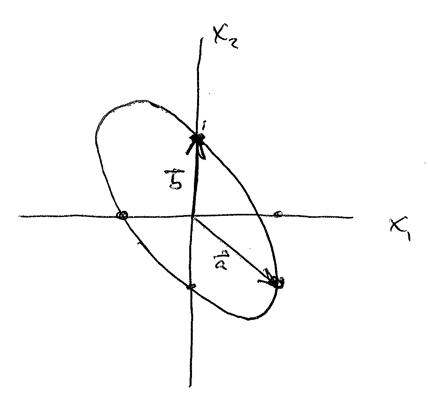
\includegraphics[scale=0.6]{26-1}\\
	{\small \textit{exercise:} how does one locate the major axis of this ellipse?}
\end{center}
\begin{equation*}
	\vec{f(t)} = \begin{bmatrix}
		1\\-1
	\end{bmatrix} \cos t -
	\begin{bmatrix}
		0\\1
	\end{bmatrix}\sin t
\end{equation*}
\textbf{Question 3:} So what do solutions $\vec{x}(t)$ of $\vec{x} = \begin{bmatrix}
	0 & 1\\ -2 & -2
\end{bmatrix} \vec{x}$, Look like?\\
\emph{Answer:} First, what is the effect of $\lambda$ in $\Gamma = \lambda + i \mu$?
\begin{itemize}
	\item If $\lambda = 0$, $\Gamma = i\mu$ is purely imaginary all solutions are ellipses encircling the origin. 
	\item If $\lambda < 0$, as $\vec{f(t)}$ traverses one period $\vec{x(t)}$ changes its magnitude by a factor of $e^{\lambda t} < 1$. Trajectories spiral inward
	\begin{center}
		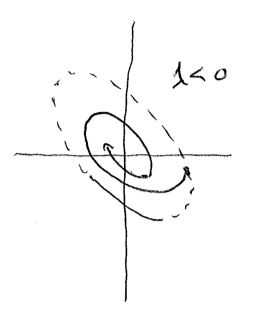
\includegraphics[scale=0.7]{26-2}
	\end{center}
	\item if $\lambda > 0$, spiral outward
	\begin{center}
		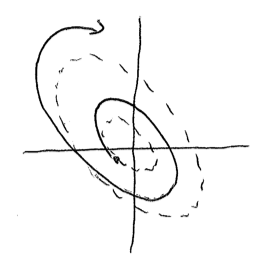
\includegraphics[scale=0.6]{26-3}
	\end{center}
	\item direction of travel?
\end{itemize}
\begin{enumerate}[label=\protect\circled{\arabic*}]
	\item Given $\vec{f(t)}$, calculate $\vec{f'(t)}$
	\item Evaluate $\vec{x}(0)$ and $\vec{x}(t)$ where $t = (\frac{2\pi}{\mu})\frac{1}{4}$ ($\frac{1}{4}$ turn around the eclipse).
\end{enumerate}
Back to stability:\\
In this case, $\Gamma_1 = \lambda + i\mu$, $\Gamma_2 = \lambda - i\mu$ as long as $\mu \neq 0$, $\Gamma_1 \neq \Gamma_2 \neq 0$. Thus the \underline{origin} is the \textbf{ONLY} equilibrium. What is its stability?
\begin{itemize}
	\item $\lambda < 0$: all solutions tend toward origin
	\item $\lambda > 0$: all solutions diverge from origin (tend toward origin or $t \rightarrow \infty$)
	\item $\lambda = 0$: Solutions are bounded and neither tend toward nor away from the origin.
\end{itemize}
\begin{example-N}
	$\vec{x}' = \begin{bmatrix}
		0 & 1\\ -2 & -2
	\end{bmatrix} \vec{x}$. Solution with $c_1 = 1$, $c_2 = 0$ is $\vec{x}(t) = e^{-t} \bigg(\begin{bmatrix}
		1\\-1
	\end{bmatrix} \cos t - \begin{bmatrix}
		0\\1
	\end{bmatrix} \sin t \bigg)$
	\begin{multicols}{2}
		\begin{enumerate}[label=\protect\circled{\alph*}]
		\item $t = 0$, $\vec{x}(t) = \begin{bmatrix}
			1\\-1
		\end{bmatrix}$
		\item $t = \frac{\pi}{2}$, $\vec{x}(t) = e^{\frac{\pi}{2}} \begin{bmatrix}
			0\\-1
		\end{bmatrix}$
	\end{enumerate}
	\end{multicols}
	\begin{center}
		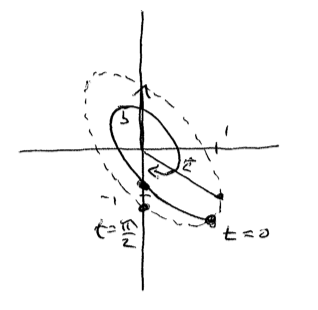
\includegraphics[scale=0.6]{26-4}
	\end{center}
\end{example-N}
For $\vec{x} = \mathbb{P}(t) \vec{x}$
\begin{definition}
	An equilibrium solution $\vec{p}$ is called \underline{asumptotically stable} if $\exists \epsilon > 0$ such that for all solutions $\vec{x}(t)$, with $\vec{x}(t_0) = \vec{x}^0$, we have
	\begin{center}
		If $|| \vec{x}^0 - \vec{p}|| < \epsilon$, then $\Lim{t \rightarrow \infty} \vec{x}(t) = \vec{p}$
	\end{center}
\end{definition}
\textbf{Notes}
\begin{enumerate}[label=\protect\circled{\arabic*}]
	\item Anything that starts within $\epsilon$ of $\vec{p}$ is asymptotic to $\vec{p}$ as $t \rightarrow \infty$.
	\item For a linear system, if $\exists\epsilon > 0$ that works then \underline{any} $\epsilon > 0$ will work (why?)
	\item An asymptotically stable equilibrium is called a \underline{sink}
\end{enumerate}
\begin{definition}
	An equilibrium solution $\vec{p}$ is called \underline{stable} if for every $\epsilon > 0$, there exists a $\delta > 0$ such that for all solutions $\vec{x}(t)$, where $\vec{x}(t_0) = \vec{x^0}$, we have
	\begin{center}
		If $|| \vec{x}^0 - \vec{p}|| < \delta$, then $||\vec{x}(t) - \vec{p}|| < \epsilon$ \qquad $\forall t \geq t_0$
	\end{center}
\end{definition}
\textbf{Notes} 
\begin{enumerate}[label=\protect\circled{\arabic*}]
	\item Given an $\epsilon$-neighborhood of $\vec{p}$ if you can always find a smaller neighborhood (a $\delta$-neighborhood) of $\vec{p}$ so that if you start in the $\delta$-neighborhood you never leave the $\epsilon$-neighborhood, then $\vec{p}$ is \underline{stable}
	\item Any $\vec{p}$ which is asymptotically stable is also stable. But only sinks are asymptotically stable
	\item An unstable equilibrium which is backward asymptotically stable (as $t \rightarrow \infty$) is called a \underline{source}
	\item For $\vec{x}' = A_{2x2} \vec{x}$, with $\Gamma_1 = \lambda + i \mu$, $\Gamma_2 = \lambda - i \mu$, $\mu \neq 0$ if $\lambda = 0$, (so that trajectories are ellipses), then $\vec{0}$ is called a \underline{centre}
\end{enumerate}
\begin{center}
	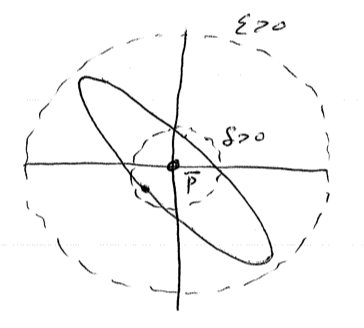
\includegraphics{26-5}
\end{center}